\documentclass[letterpaper]{article}
\usepackage{natbib,alifeconf}
\usepackage[breaklinks=true]{hyperref}
\usepackage{url}
\usepackage{graphicx}
\graphicspath{{../img/}}
\DeclareGraphicsExtensions{.pdf}

\title{EvoDraw: Interactive Evolution of Animations}
\author{ Mario Garc\'ia-Valdez, Alejandra Mancilla, Georgina Aguilar, Juan-J.~Merelo$^1$\\
\mbox{}\\
Dept. of Graduate Studies at Instituto Tecnol\'ogico de Tijuana \\
$^1$Dept. of Computer Architecture and Technology and CITIC, 
University of Granada \\
{\tt mario@tectijuana.edu.mx},{\tt jmerelo@ugr.es}}

\begin{document}
\maketitle


\section{Introduction} 

Evolutionary Algorithms (EAs) were conceived as heuristic techniques 
capable of addressing hard optimization problems 
\citep{DBLP:books/daglib/0015527}. But their possibilities as a source of
creativity were soon appreciated and applied to art, design and music \citep{ie1}, including generative design and
art \citep{Bentley:1999:intro,Sims:1991,todd:1992}.  A particular problem in
these systems is how to evaluate the quality of individuals within the population
when aesthetic quality is considered, since it is difficult to
accurately define a function that measures aesthetics. Therefore, researchers
have resorted to humans to perform this specific task, thus defining Interactive
Evolutionary Algorithms (IEAs): standard EAs whose fitness evaluations are
performed by human beings in an interactive fashion. Examples of web-based IEAs are
those by \cite{picbreeder} and \cite{forms}
use  to evolve artistic artifacts using a generative encoding, compositional
pattern producing networks, both presented on the web.
%In IEAs the main evolutionary loop includes the human intervention for quality assessment of evolved solutions. 
% JJ- this is reiterative 
There is an inherent drawback in the human fatigue caused by the repeated evaluation, and some authors have
already tried to address this \citep{Frade:2010:EvoGAMES}, for instance simplifying the interface to show a single button \cite{Davies2016}. %how? - JJ
%  Both works offer webpages (see Picbreeder.org and
% EndlessForms.com), where users can select or create random individuals and
% evolve lineages of artifacts based on their preferences.
% JJ - also a bit reiterative

The present installation builds on a previous work \citep{garcia2013evospace}
but this version is directly inspired by the 1997 Galápagos interactive 
media installation by \cite{galapagos} that allowed visitors to evolve 3D animated forms. 
In Gal{\'a}pagos twelve computers displayed simulations of growth and 
behavior of a population of abstract animated forms. Viewers
participate in this exhibit by selecting which organisms they find
most aesthetically interesting by standing on step sensors in front 
of those displays. The selected organisms survive, mate, mutate and 
reproduce. EvoDraw is also an IEA where through the interaction
with viewers, animations are selected. Animations are inspired in 
the Process Compendium by \cite{reas:2004}, where visual forms 
emerge by the relations of multiple forms and their behavior. 

\label{Description}
\begin{figure*}[!t]
\centering
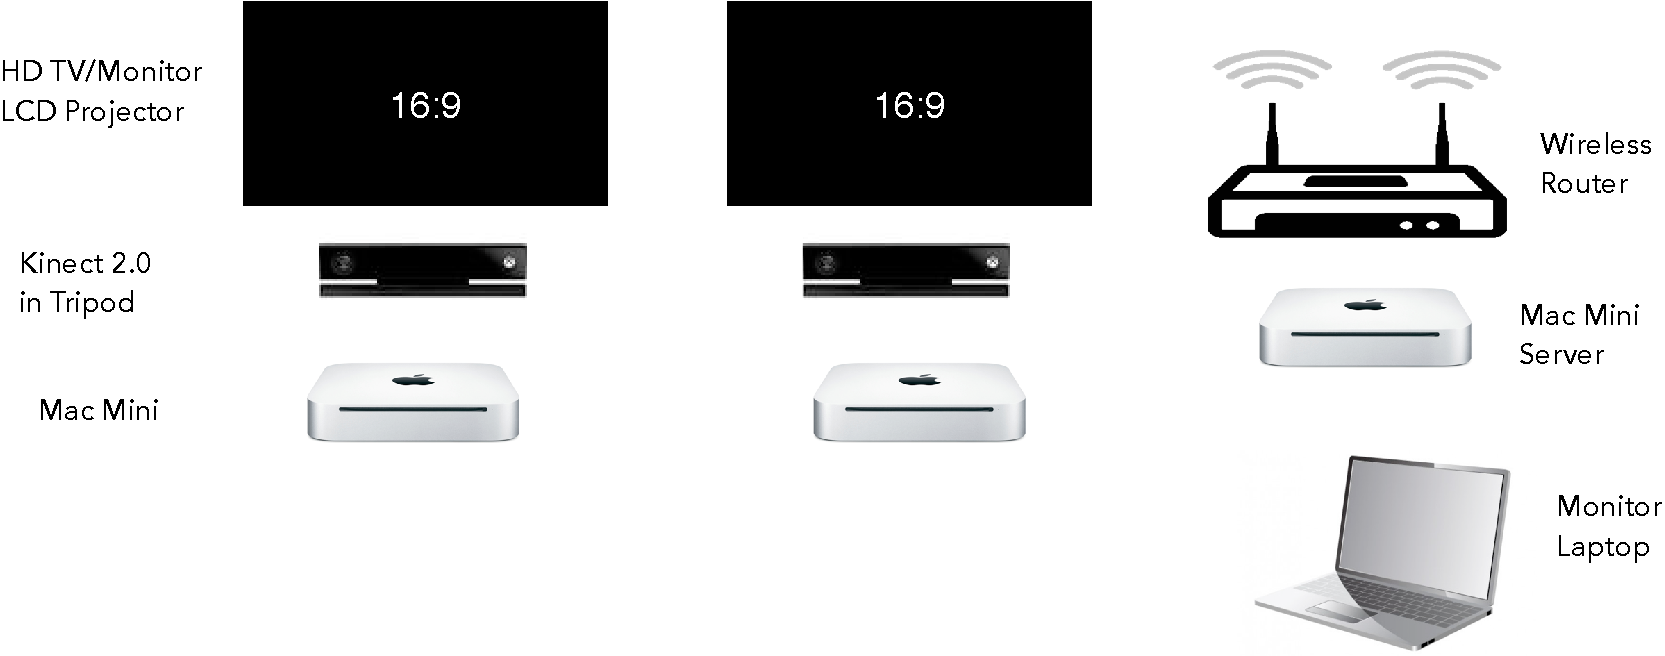
\includegraphics[width=6in]{EvoDrawTech.pdf}
\caption{Proposed setup}
\label{fig:system}
\end{figure*}

\section{Description of the Artistic Project} 
The EvoDraw installation is an IEA in which viewers interact with animations by simply
looking at them. Drawings emerge from animations scripted in the Processing 
language, and each is configured by a list of parameters represented by their
chromosome. To start the evolutionary cycle, first a population of animations is 
randomly generated and stored in a container server called EvoSpace. Once the population is active, 
client computers remove animations from the evospace server to be presented in a monitor
one at a time. After a certain amount of time, animations are put back to the server along 
with information generated from the interaction. To continue, another is again removed and presented
to viewers. An important feature is that once an animation is removed from the server,
no other client can remove it, until the client that remove it puts the animation back, this means that any
animation is been shown only
on one client at a given time. This cycle continues until there is enough interactions to create a new
generation of animations. In the previous version of this system \citep{garcia2013evospace} 
viewers directly assigned a rating to each animation via a web page; in this work, viewers
only need to see the animations on different monitors, but this time they can look at them or not, just like
the paintings inside a gallery. In order to assign a fitness value to each animation and thus 
enabling the EA the selection of the more interesting animations, 
a natural user interface device (Kinect sensor for Xbox One)
is used for facial tracking. The sensor can track up to 6 persons at once and  
it provides a basic set of information for every face: where the face is, where it is looking, 
basic expressive information, and if the face has glasses, which are used to compute the attention received by each simulation. Each animation is 
presented several times in a single generation and the best are always passed to the next, with its fitness recomputed. To generate the new population GA operators
are applied to the population. One or more client computers are needed in order to run the 
installation, each needing a Kinect sensor to keep track of viewers. 
% Other interfaces to
% the system could be combined, for instance to allow user with a smart-phone to directly assign
% a rating to each animation or to see their genetic ancestry.
% JJ this is more future work. 
\section{Technical Elements of the Installation}
The hardware components of the installation are presented in Figure \ref{fig:system}. A
minimum of one station is needed. Each stations consists of a small computer, needed 
to run the Kinect application and to show a web page where the animation is displayed, 
a Kinect sensor mounted in a tripod and a monitor or LCD projector appropriate to the
size of the venue. Another computer is needed to act as the server. Currently four stations
and server are available for the installation.  

One of the  goal of this work is to develop an open source framework for Web and local
IEA systems, using current web standards and libraries for mobile devices and to explore 
innovative ways in which users can be part of the IEA algorithm. All the code of this work
is available as open source from \url{https://github.com/mariosky/evospace-js}. 













\bibliographystyle{apalike}
\bibliography{evospace-i}

\end{document}
